\newpage % Zaleca się otwieranie rozdziału od nowej strony.
\section{Zagadnienie kinematyki odwrotnej dla platformy}

% In industry and science often hydraulic Stewart Platforms are deployed for their robustness, fast acceleration and retention force, but only few publications focus on a cheap design using electric motors. In recent years many hobbyists built Stewart Platforms, but either they are not documented well or they are built to have a proof of concept without much theory behind. With this article I want to close this gap, derive the inverse kinematics of the Stewart Platform using cheap servo motors and provide a software library to visualize and build own platforms.


\subsection{Czym jest kinematyka odwrotna?}
%The inverse kinematics of a Stewart Platform is the calculation of the leg length given the required position of the platform. The forward kinematic is not distinct and can only be determined with additional constraints or sensor input and is not covered here.
%The Stewart Platform consists of two frames, the base frame and the platform frame that are connected with six variable length legs. With this setup the platform can be moved in three translational dimensions and three rotational dimensions.
Zadanie kinematyki odwrotnej polega na obliczeniu potrzebnej długości nóg platformy, aby uzyskać zadaną pozycje platformy. 
W przypadku klasycznej konstrukcji platformy z liniowymi aktuatorami wyniki można w prosty sposób wykorzystać w programie, jednak w przypadku nóg zbudowanych na bazie serw, trzeba dodać kolejny krok, czyli obliczenie określonego kąta ramienia serwomechanizmu, aby uzyskać pożądaną długość nogi. 
Trzeba także zwrócić uwagę na położenie serwa i zwrot skierowania jego ramienia na płaszczyźnie X,Y w układzie współrzędnych podstawy, zakładając, że położenie na osi Z równa się wysokości, na której znajduje się wał obracany przez silnik.
\\\\
Poniżej zamieszczam zdjęcie z nałożonymi w przestrzeni punktami niezbędnymi do obliczeń kątów koniecznych do zadania aby uzyskać zadaną pozycję platformy górnej.
W celu ułatwienia obserwacji, zaznaczono punkty konieczne do obliczeń tylko jednej nogi, oznaczanej indeksem k.

% o co chodzi z tymi wektorami, jak to rozumiec?

% Miejsce na rysunek przedstawiajacy wektory opisujace translacje

\begin{figure}[!h]
    \label{fig:anzelm}
    \centering
    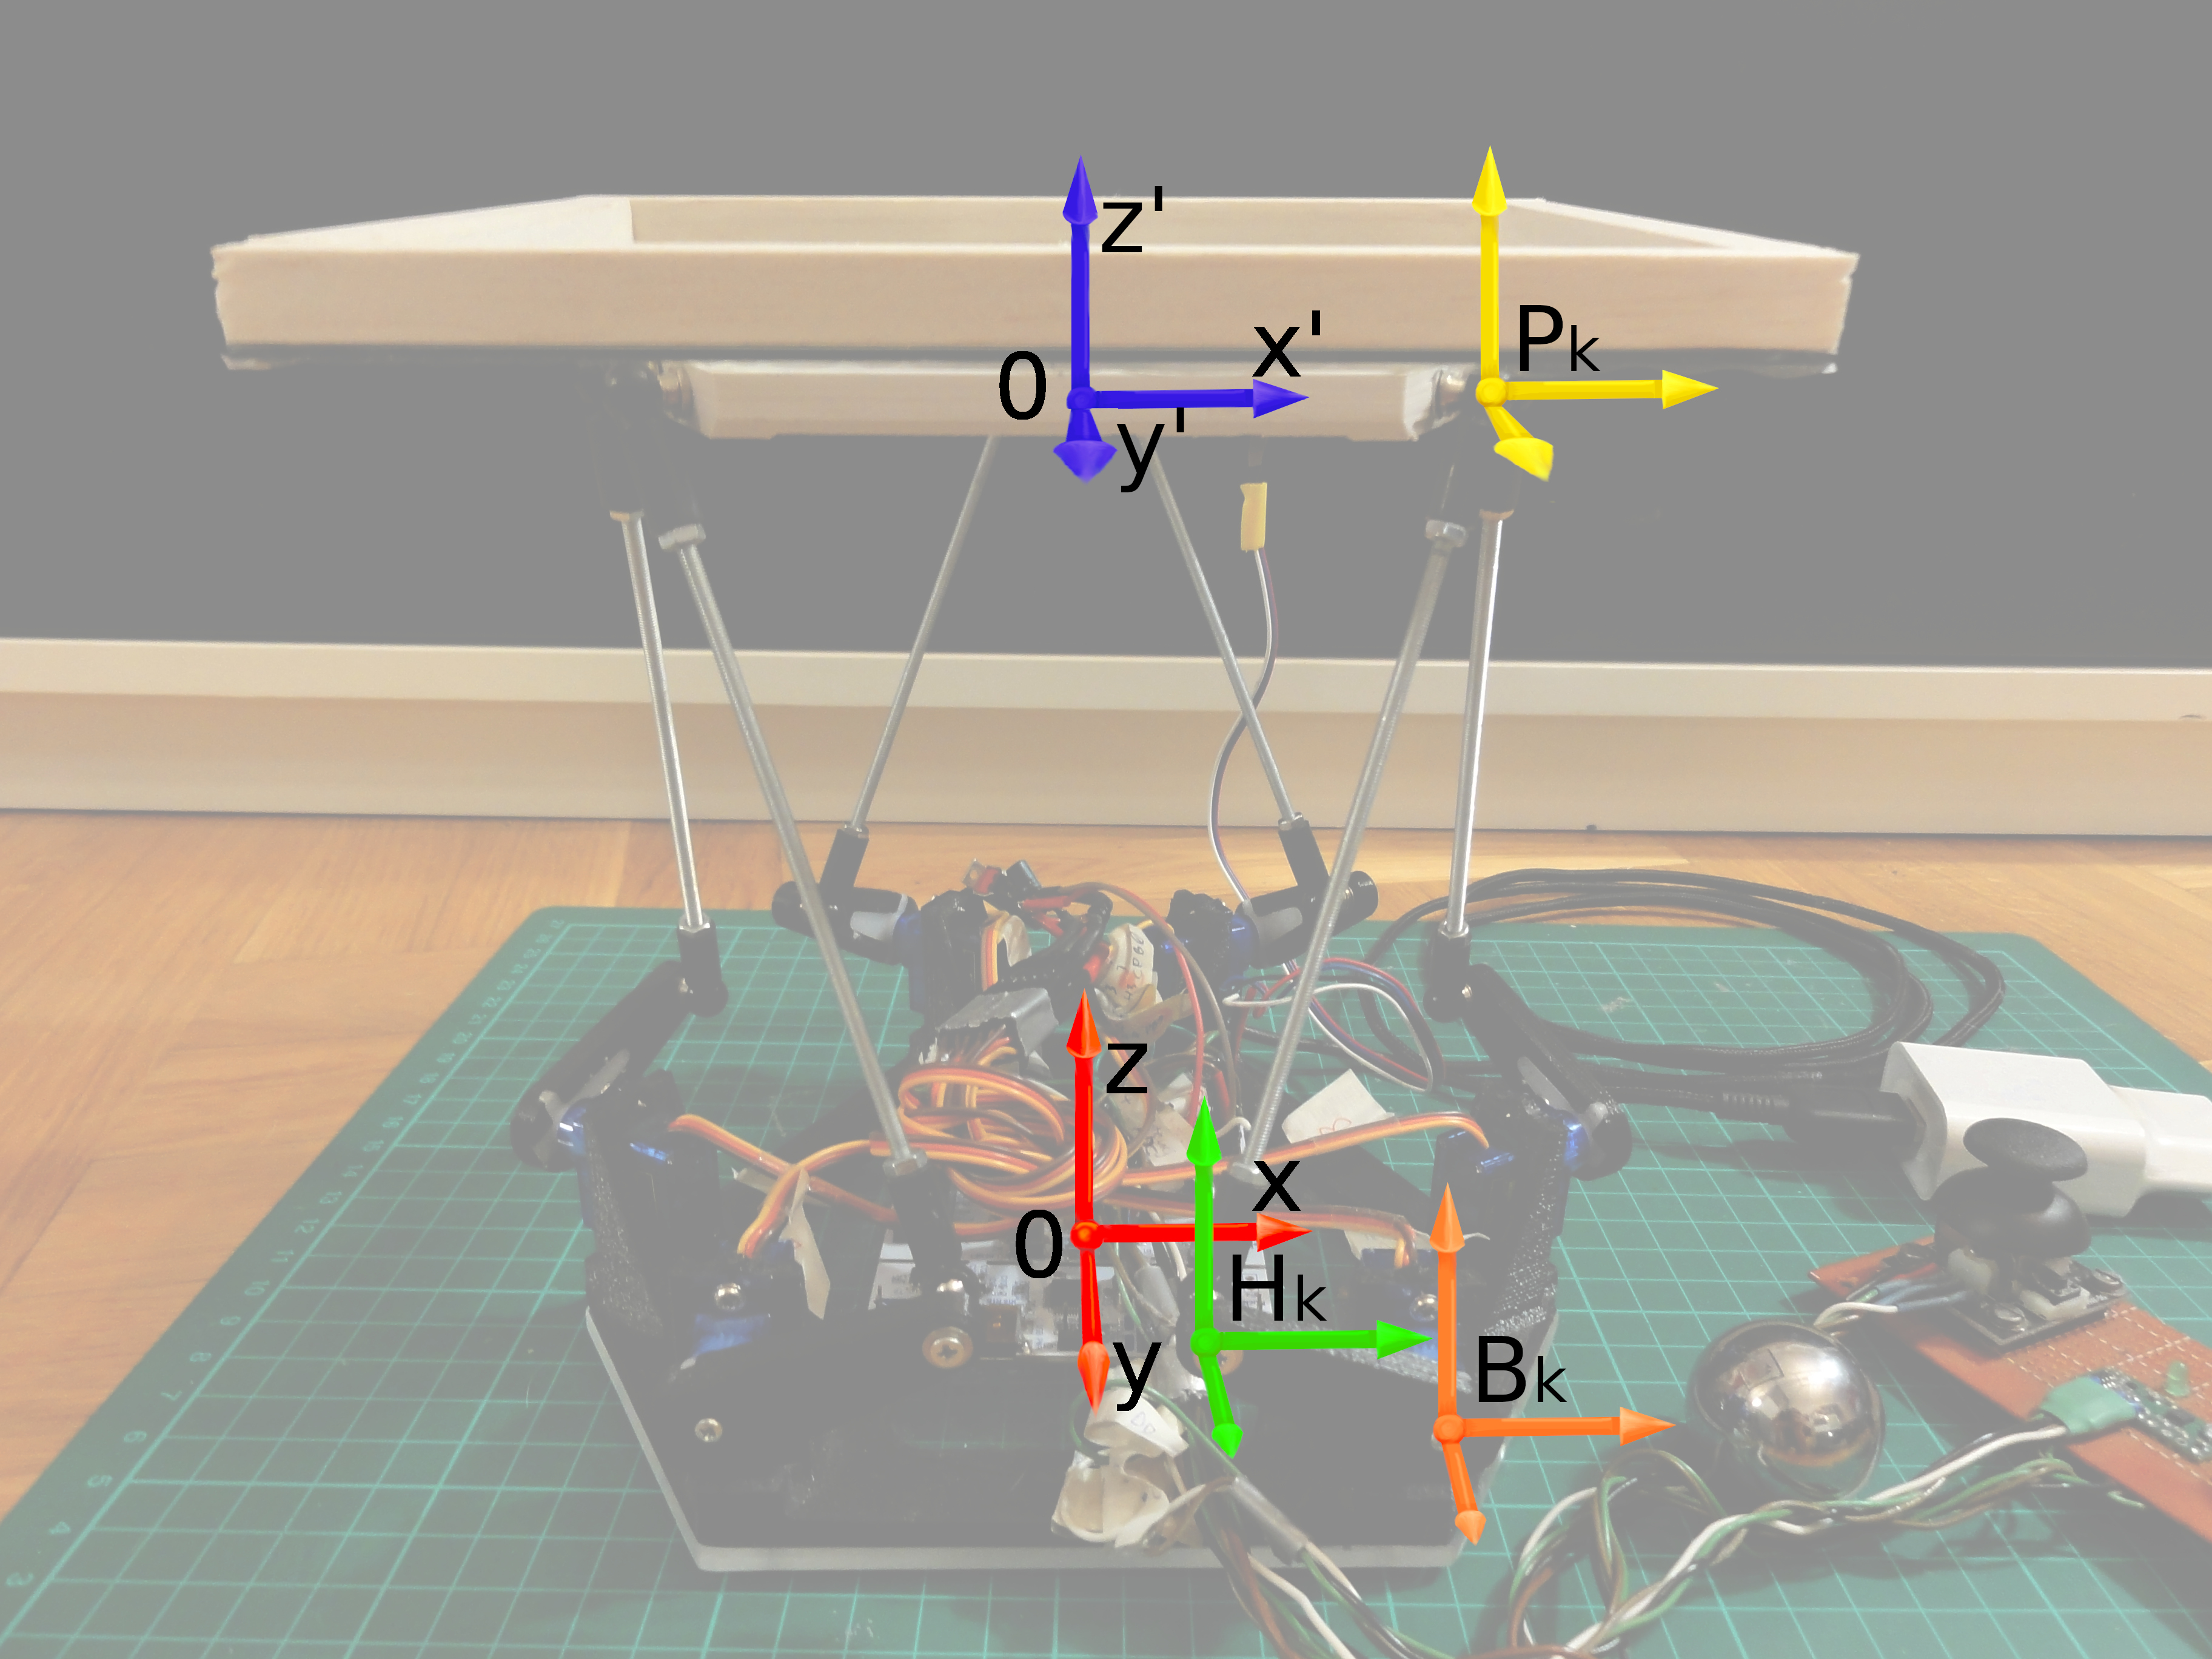
\includegraphics[width=\textwidth]{img/Platforma_rzeczywista_punkty.jpg}
    \caption{Zaznaczenie waznych ounktów do obliczeń w przestrzeni 3D.}
    % \captionsource{Źródło: }{}
\end{figure}


\subsection{Typowe obliczenia dla konstrukcji z siłownikami.}
Poniżej przedstawie relacje między układem współrzędnych talerza
$\textbf{P}\{\coord{x^{'},y^{'},z^{'}}\}$ 
od układu podstawy 
$\textbf{B}\{\coord{x,y,z}\}$ 
, z zaznaczeniem punktu bazy k-tego serwa $B_k$ i punktu przegubu górnego talerza k-tej nogi $P_k$. 

\begin{figure}[!h]
    \label{fig:anzelm}
    \centering
    % Mozna poprawic zdjecie, zeby bylo profesjonalnie zwymiarowane
    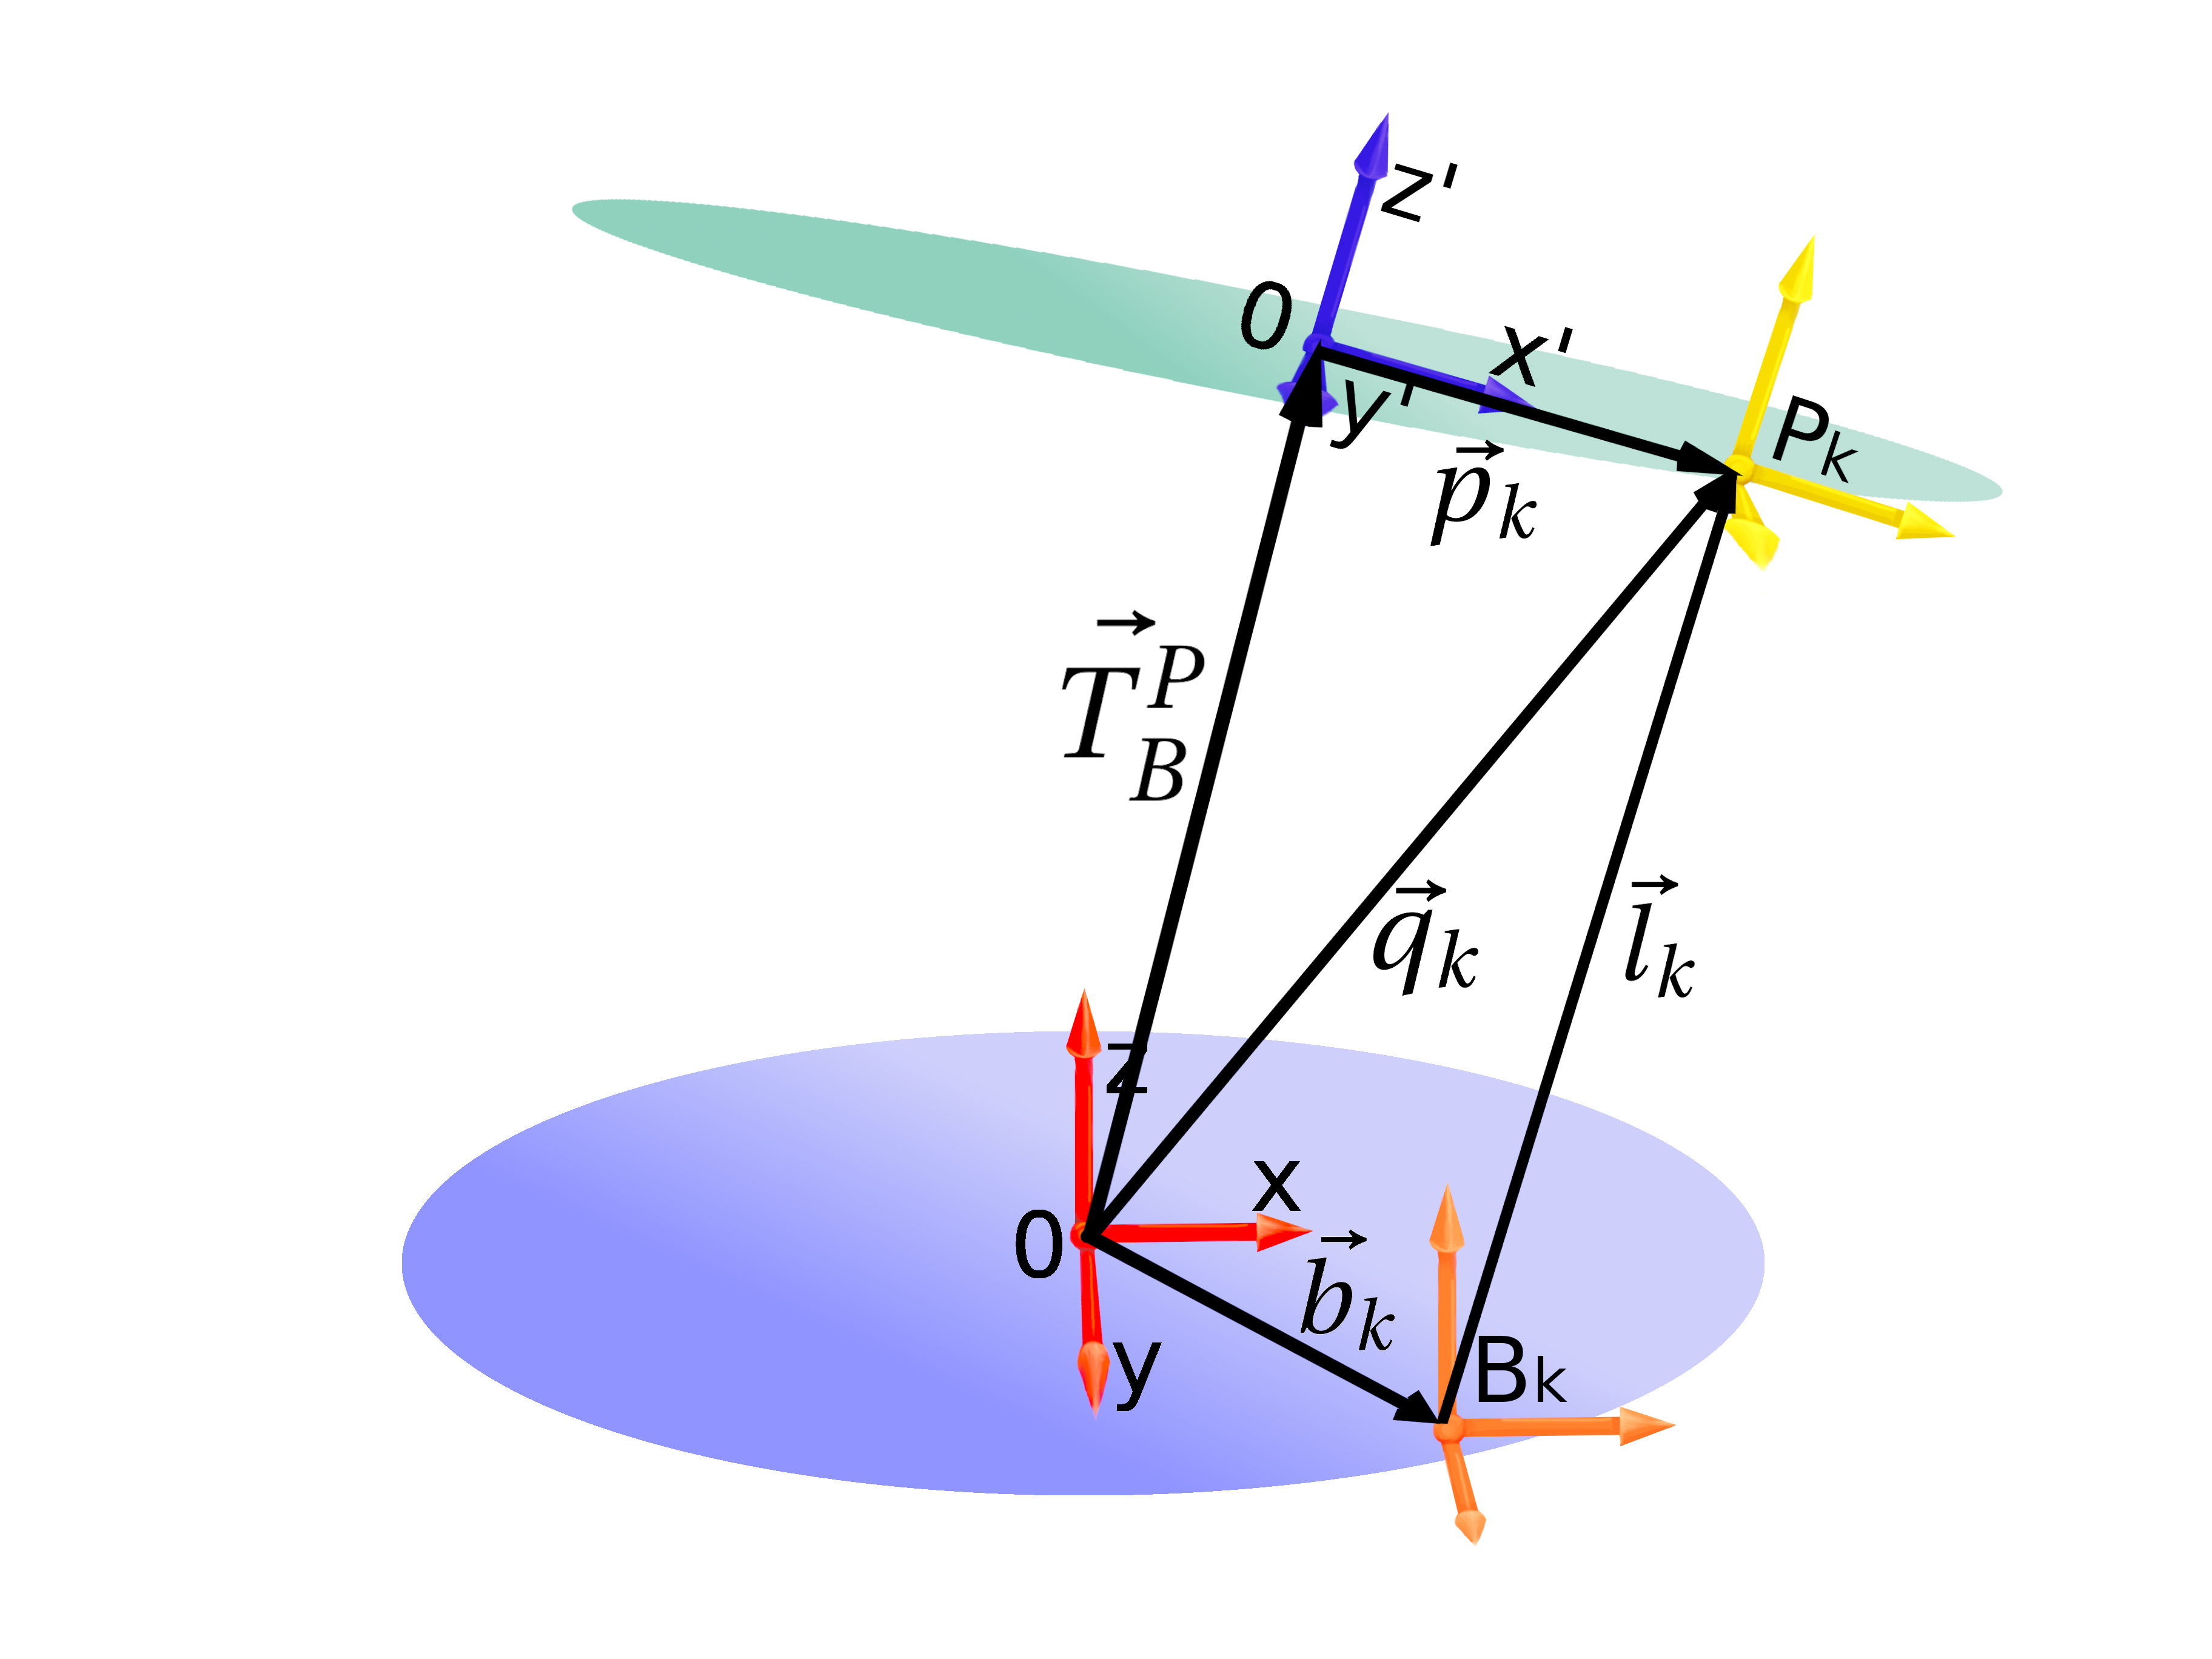
\includegraphics[width=0.5\linewidth]{img/wektory_kinematyka.png}
    \caption{Wektory opisujące przekształcenie układu współrzędnych podstawy do platformy.}
    % \captionsource{Źródło: }{}
\end{figure}

,gdzie: \\ % Wyjasnienie co opisuja te wektory:
${\vec{b_k}}$ - wektor położenia punktu bazy serwa k-tej nogi $B_k$ w układzie współrzędnych bazy $\textbf{B}\{\coord{x,y,z}\}$, \\ 
${\vec{q_k}}$ - wektor położenia punktu górnego przegubu k-tej nogi w bazowym układzie współrzędnych, \\  
${\vec{p_k}}$ - wektor położenia punktu górnego przegubu k-tej nogi w układzie współrzędnych platformy $\textbf{P}\{\coord{x^{'},y^{'},z^{'}}\}$ , \\ 
${\vec{l_k}}$ - wektor opisujące położenie punktu $P_k$ względem punktu $B_k$ w bazowym układzie współrzędnych. \\
${\vec{T_P^{B}}}$ - wektor opisujący położenie punktu zerowego układu współrzędnych platformy względem punktu zerowego układu współrzędnych bazowych.
\\
Z wyznaczonych wektorów i uwzględniając macierz Transformacji układu $\textbf{P}\{\coord{x^{'},y^{'},z^{'}}\}$ względem $\textbf{B}\{\coord{x,y,z}\}$

$\Trans^{P}_{B} = $
\[
\begin{bmatrix}
1 & 1 & 1 \\
1 & 1 & 1 \\
1 & 1 & 1
\end{bmatrix}
\]



\begin{figure}[!h]
    \label{fig:anzelm}
    \centering
    % Mozna poprawic zdjecie, zeby bylo profesjonalnie zwymiarowane
    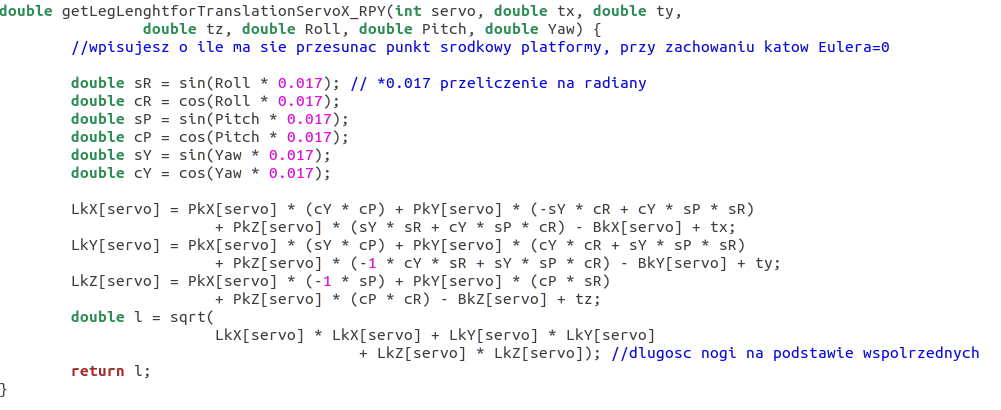
\includegraphics[width=\textwidth]{img/kod_inverse_kinematics_1.png}
    \caption{Metoda obliczenia długości nóg potrzebnych do uzyskania pozycji.}
    % \captionsource{Źródło: }{}
\end{figure}


\subsection{Uwzględnienie konstrukcji opartej na serwomechanizmach.}
\begin{figure}[!h]
    \label{fig:anzelm}
    \centering
    % Mozna poprawic zdjecie, zeby bylo profesjonalnie zwymiarowane
    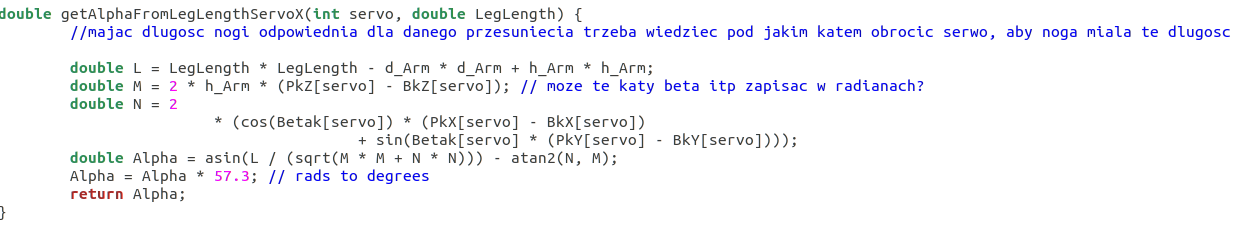
\includegraphics[width=\textwidth]{img/kod_inverse_kinematics_2.png}
    \caption{Metoda obliczenia kąta do zadania na serwo, aby uzyskać określoną długość nogi.}
    % \captionsource{Źródło: }{}
\end{figure}


\subsection{Funkcja ustawiająca platformę w zadanym położeniu.}
\begin{figure}[!h]
    \label{fig:anzelm}
    \centering
    % Mozna poprawic zdjecie, zeby bylo profesjonalnie zwymiarowane
    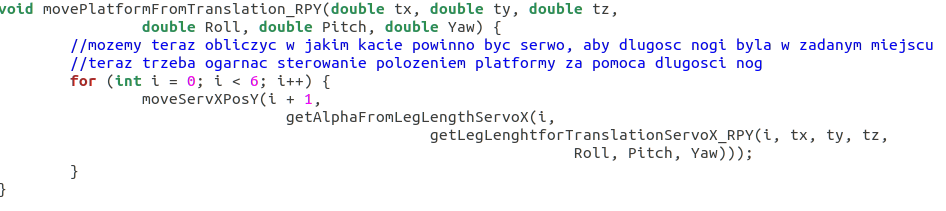
\includegraphics[width=\textwidth]{img/kod_inverse_kinematics_3.png}
    \caption{Metoda ruchu.}
    % \captionsource{Źródło: }{}
\end{figure}



\begin{figure}[!h]
    \label{fig:anzelm}
    \centering
    % Mozna poprawic zdjecie, zeby bylo profesjonalnie zwymiarowane
    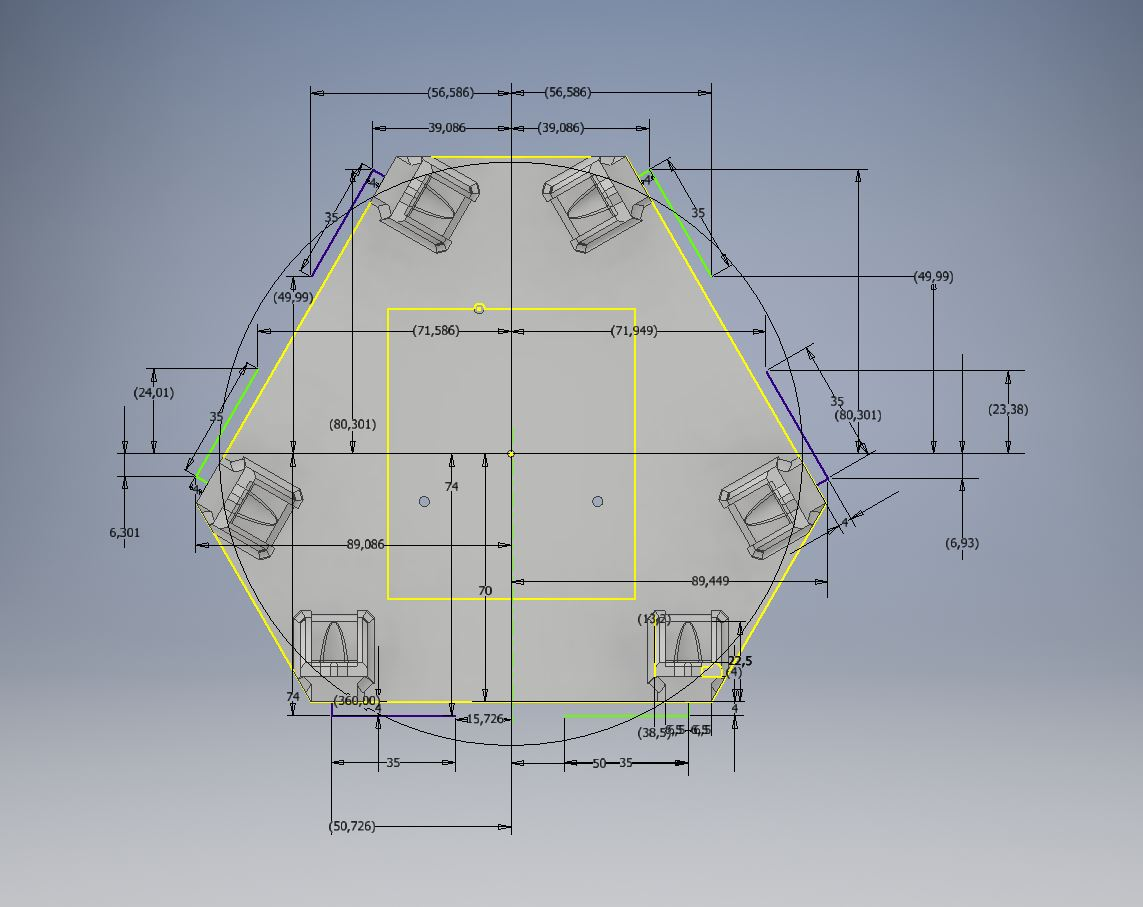
\includegraphics[width=0.5\linewidth]{img/Base_2D_messy.JPG}
    \caption{Szkic 2D platformy z wymiarami.}
    % \captionsource{Źródło: }{}
\end{figure}

\subsection{Przeksztalcanie wzorow i dojscie do wyniku}

\subsection{Zdjecia przykładowej metody}

% {\Large 
% $
% {\vec{b_k}} \\ 
% {\vec{T}}    \\   
% {\vec{q_k}}  \\  
% {\vec{p_k}}  \\ 
% {\vec{l_k}} \\
% {\vec{T_B^{P}}} \\
% {\vec{T_P^{B}}}
% $ \par}